\subsection{Data Structures of Tree RCU} \label{sec:data_structure}
% In Section~\ref{sec:rcu_softirq}, we discuss how RCU's softirq handlers walk up the 
% tree hierarchy of the \co{rcu_node} data structure. In ths section, we explain 
% in detail how this data structure is implemented in \co{kernel/rcu/tree.h} and used 
% in Tree RCU.

\begin{figure}[tbp]
\centering
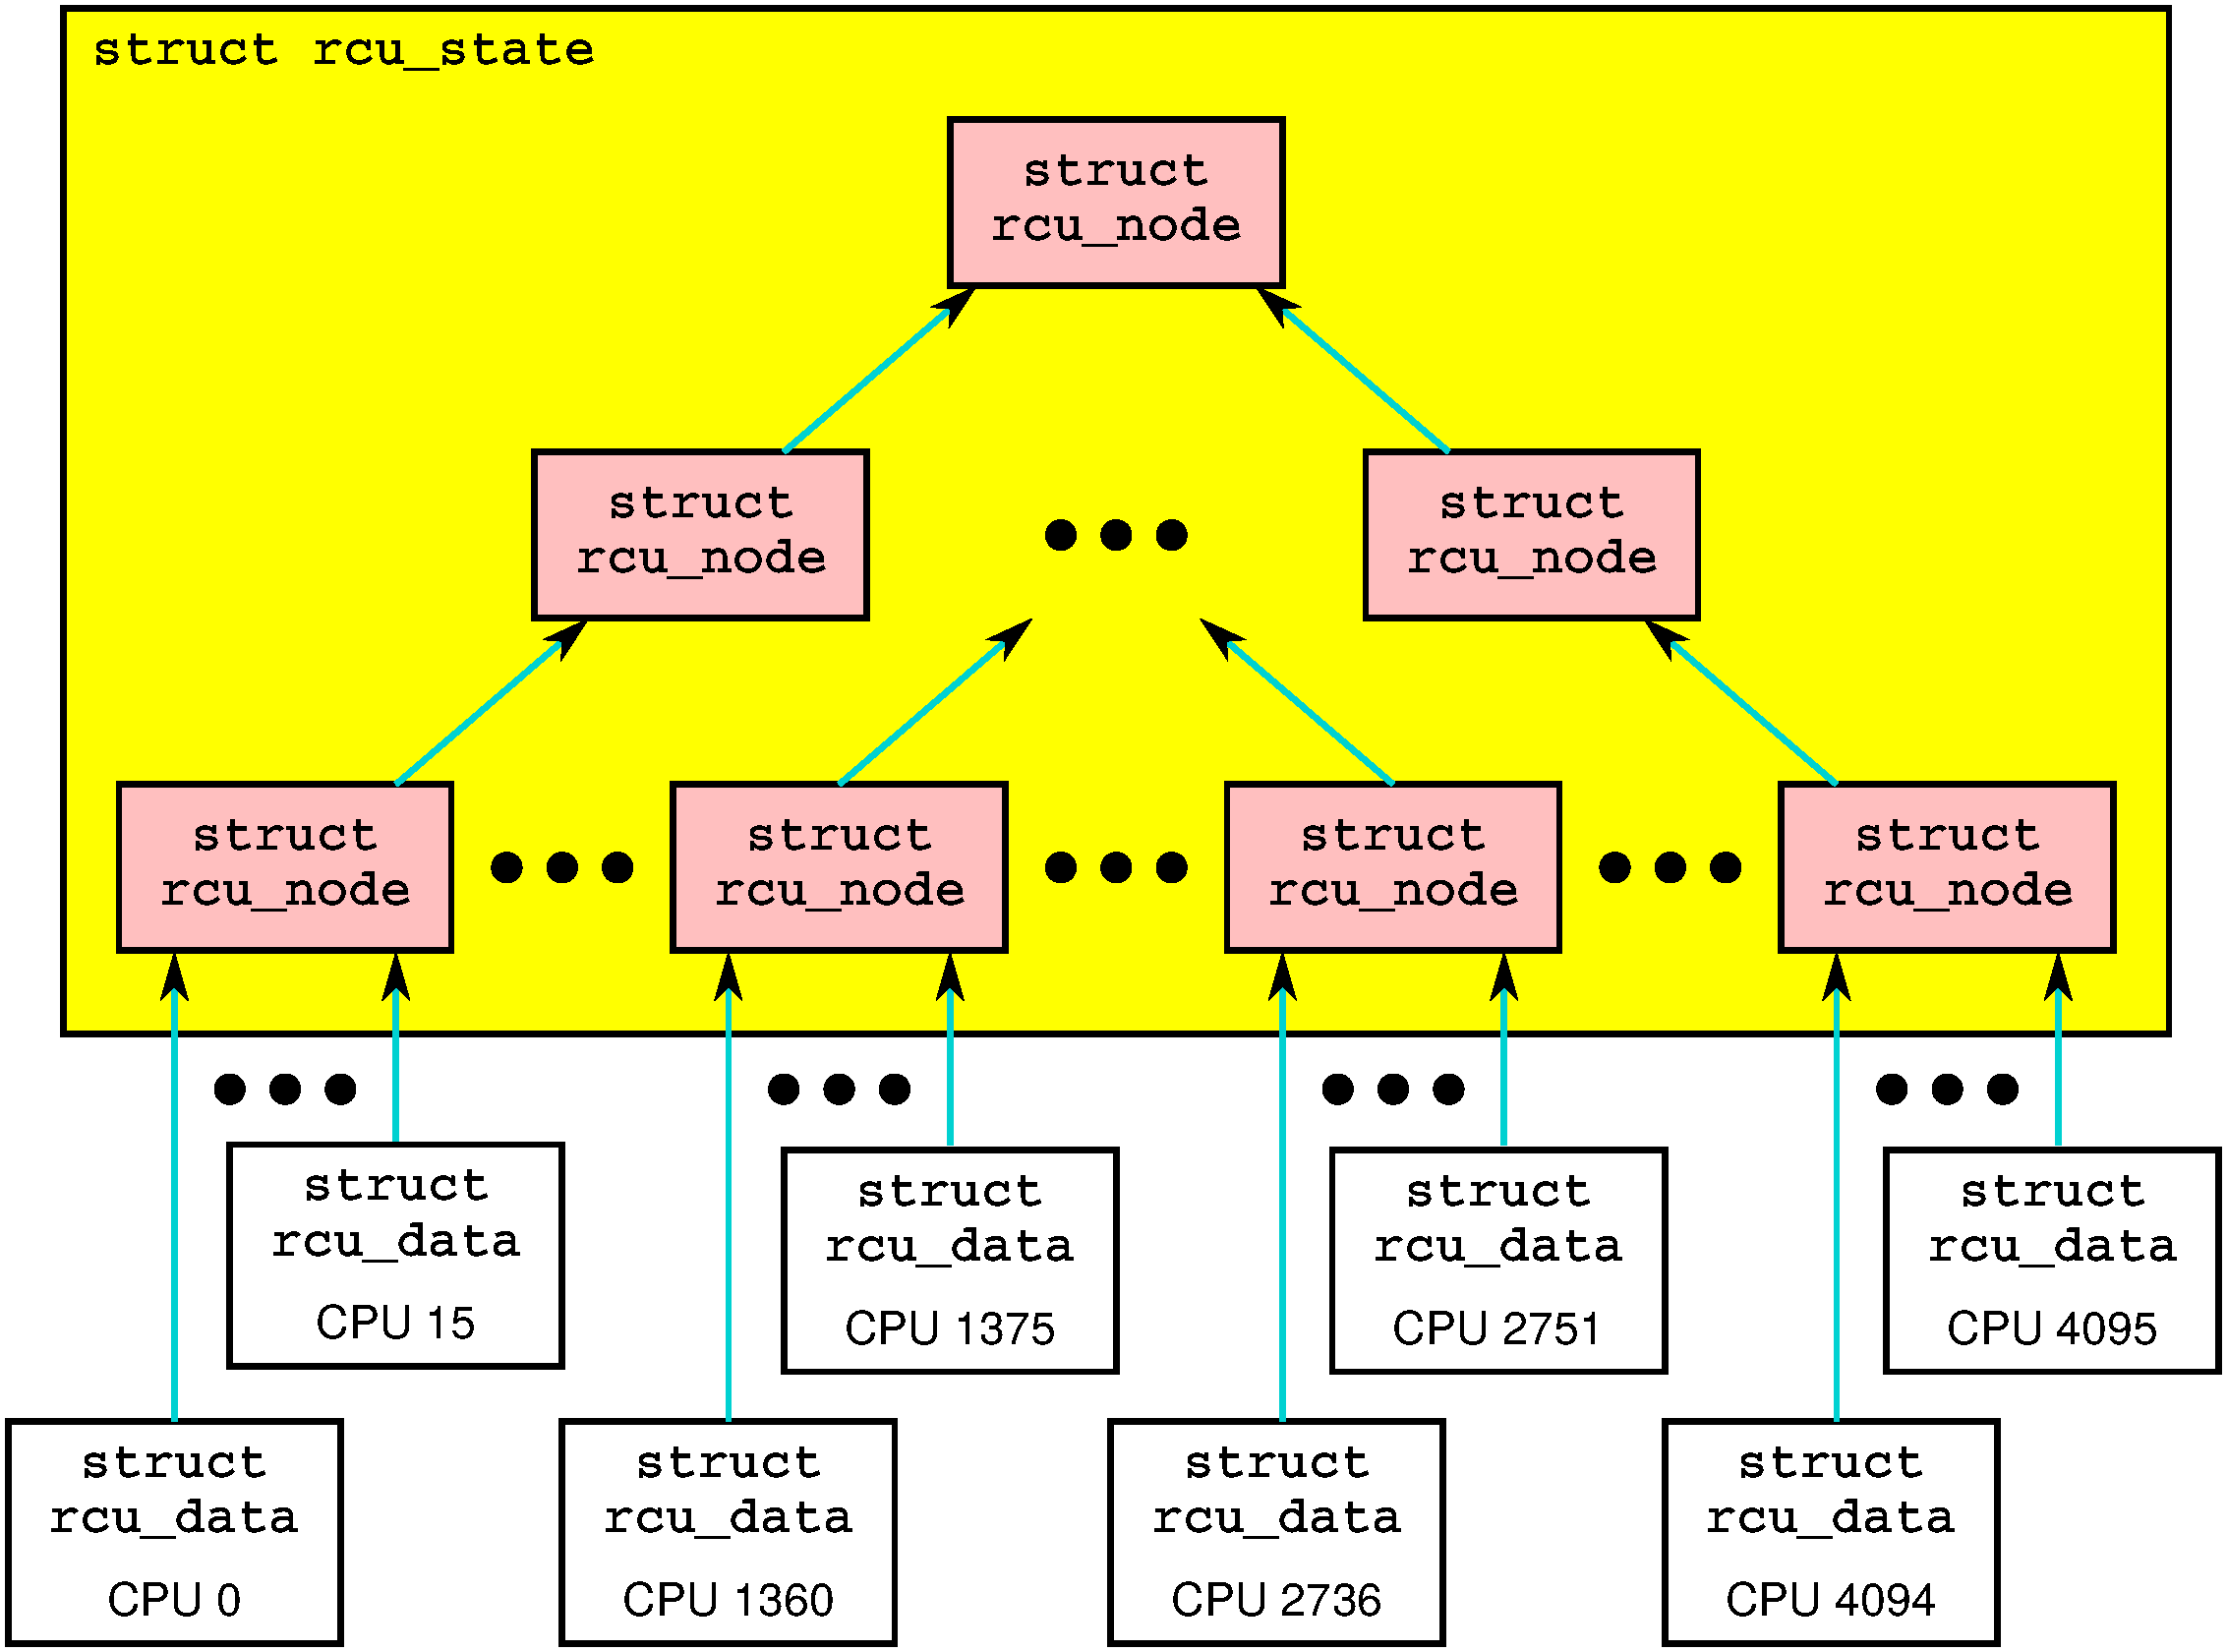
\includegraphics[scale=0.2]{tree_rcu_hierarchy.pdf}
\caption{Tree RCU Hierarchy}
\label{fig:tree_rcu_hierarchy}
\end{figure}

RCU's global state is recorded in the \co{rcu_state} structure, which consists of 
a tree of \co{rcu_node} structures with a child count of up to 64
(32 in a 32-bit system). Every leaf node can have at most 64 
\co{rcu_data} structures (again 32 on a 32-bit system), each representing
a single CPU, as illustrated in
Figure~\ref{fig:tree_rcu_hierarchy}.
%
Each \co{rcu_data} structure records its CPU's quiescent states, and
the \co{rcu_node} tree propagates these states up to the root, and then
propagates grace-period information back down to the leaves.
%
Quiescent-state information does not propagate upwards from a given node
until a quiescent state has been reported by each CPU covered by the subtree
headed by that node.
This propagation scheme dramatically reduces the lock contention experienced
by the upper levels of the tree.
%
% Lihao: include this in PhD thesis and the technical report
For example, consider a default \co{rcu_node} tree for a 4,096-CPU system,
which will have have 256 leaf nodes, four internal nodes, and one root node.
During a given grace period, each CPU will report its quiescent states
to its leaf node, but there will only be 16 CPUs contending for each of
those 256 leaf nodes.
Only 256 of the CPUs will report quiescent states to the internal nodes,
with only 64 CPUs contending for each of the four internal nodes.
Only four CPUs will report quiescent states to the root node, resulting
in extremely low contention on the root node's lock, so that contention
on any given \co{rcu_node} structure is sharply bounded even in very
large configurations.
%
The current RCU implementation in the Linux kernel supports up to a
four-level tree, and thus in total $64^4 = 16,777,216$ CPUs in a 64
bit machine.\footnote{
	Four-level trees are only used in stress testing,
	but three-level trees are used in production by 4096-CPU systems.}

\subsubsection{\co{rcu_state} Structure}

\begin{figure}[tbp]
\centering
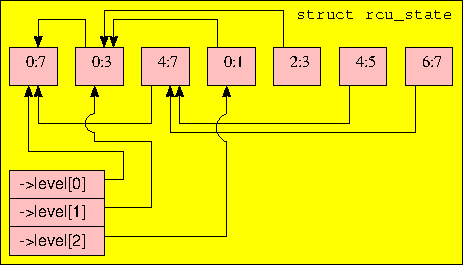
\includegraphics[scale=0.9]{rcu_node_array.pdf}
\caption{Array Representation for a Tree of \co{rcu_node} Structures}
\label{fig:rcu_node_array}
\end{figure}

Each flavor of RCU has its own global \co{rcu_state} structure. 
%For example, \co{rcu_state} pointers \co{rcu_sched_state}, 
%\co{rcu_bh_state} and \co{rcu_state_p} are used by RCU-sched, RCU-bh 
%and RCU-preempt, respectively. 
The \co{rcu_state} structure includes
a array of \co{rcu_node} structures organized as a tree
\co{struct rcu_node node[NUM_RCU_NODES]}, with
\co{rcu_data} structures connected to the leaves.
Given this organization, a breadth-first traversal is 
simply a linear scan of the array.
%\comment{Lihao: we may also remove the following sentence and the figure 
%as it's a bit too technical and the level array is never refered again in the paper}
% Lihao: include this in the technical report
Another array \co{struct rcu_node} \co{*level[NUM_RCU_LVLS]} 
is used to point to the left-most node at each level of the tree,
as shown in Figure~\ref{fig:rcu_node_array}.

The \co{rcu_state} structure uses \co{unsigned long} fields \co{->gpnum}
and \co{->completed} to track RCU's grace periods.
The \co{->gpnum} field records the most recently started grace period,
whereas \co{->completed} records the most recently ended grace period.
If the two numbers are equal, then corresponding flavor of RCU is idle.
If \co{gpnum} is one greater than \co{completed}, then RCU is in the
middle of a grace period.
All other combinations are invalid.
% Which of course means that we could instead use a single counter with an
% odd/even scheme to track grace periods.

%(Lihao: ignore variables used to force quiescent states by force_quiescent_state())

\subsubsection{\co{rcu_node} Structure}
\label{sec:rcu_node}
The tree of \co{rcu_node} structures records and 
propagates quiescent-state information from the leaves to the root,
and also propagates grace-period information from the root to the leaves. 
%
The \co{rcu_node} structure has a spinlock \co{->lock} to protect its fields.
The \co{->parent} field references the parent \co{rcu_node} structure,
and is \co{NULL} for the root.
The \co{->level} field indicates the level in the tree, counting from zero
at the root.
The \co{->grpmask} field identifies this node's bit in the
\co{->qsmask} field of its parent.
The \co{->grplo} and \co{->grphi} fields indicates the lowest and highest 
numbered CPU that are covered by this \co{rcu_node} structure, respectively.

The \co{->qsmask} field indicates which of this node's children
still need to report quiescent states for the current grace period.
%
As with \co{rcu_state}, the \co{rcu_node} structure has \co{->gpnum} 
and \co{->completed} fields that have values identical to those of the
enclosing \co{rcu_state} structure, except at the beginnings and ends
of grace periods when the new values are propagated down the tree.
Each of these fields can be smaller than 
its \co{rcu_state} counterpart by at most one.

%\comment{Lihao: comment out the following preemptible RCU contents if we need space.}
%In a preemptible kernel, tasks can be preempted during RCU read-side
%critical sections.
%When an RCU read-side critical section is preempted,
%the preempted task's \co{task_struct} is enqueued onto the \co{->blkd_tasks}
%list in the leaf \co{rcu_node} structure covering the task's CPU.
%That task will remove itself once it reaches the RCU read-side critical
%section's outermost \co{rcu_read_unlock()},
%%
%When the \co{->gp_tasks} pointer is non-\co{NULL}, it references the first
%task blocking the current grace period.
%When a task referenced by \co{gp_tasks} points is removed 
%from \co{blkd_tasks}, the pointer will be advanced to the next task on the list,
%or is set to \co{NULL} if there are no more tasks.
%Note that
%tasks blocking the current grace period are queued in the reverse time order.
%Thus, if a task is blocking a grace period, 
%all subsequent tasks on the list are blocking the same grace period.
% Lihao: how the tasks are dequeued is described in quiescent state detection
% Lihao: we ignore expedited grace period for now
% Lihao: we don't model priority boosting

\subsubsection{\co{rcu_data} structure} \label{sec:rcu_data}
The \co{rcu_data} structure detects quiescent states and handles RCU
callbacks for the corresponding CPU.
The structure is accessed primarily from the corresponding CPU,
thus avoiding synchronization overhead.
As with the \co{rcu_state} structure, different flavors of RCU maintain 
their own per-CPU \co{rcu_data} structures. %For instance, RCU-sched's 
%\co{rcu_sched_state}, RCU-bh's \co{rcu_bh_state} and RCU-preempt's 
%\co{rcu_state_p} structures have \co{rcu_data} structures \co{rcu_sched_data}, 
%\co{rcu_bh_data}, and \co{rcu_data_p}, respectively.
%
The \co{->cpu} field identifies the corresponding CPU, the \co{->rsp}
field references the corresponding \co{rcu_state} structure, and the
\co{->mynode} field references the corresponding leaf \co{rcu_node}
structure.
The \co{->grpmask} field identifies this \co{rcu_data} structure's bit
in the \co{->qsmask} field of its leaf \co{rcu_node} structure.

The \co{rcu_data} structure's \co{->qs_pending} field indicates that RCU
needs a quiescent state from the corresponding CPU, and the
\co{->passed_quiesce} indicates that the CPU has already passed through
a quiescent state.
%
The \co{rcu_data} also has \co{->gpnum} and \co{->completed} fields,
which can lag arbitrarily behind their counterparts in
the \co{rcu_state} and \co{rcu_node} structures on idle CPUs.
However, on the non-idle CPUs that are the focus of this paper,
they can lag at most one grace period behind their leaf \co{rcu_node} 
counterparts.

The \co{rcu_state} structure's \co{->gpnum} and \co{->completed} fields
represent the most current values, and are tracked closely by those of
the \co{rcu_node} structure, which allows the \co{->gpnum} and
\co{->completed} fields in the \co{rcu_data} structures to be
are compared against their counterparts in the corresponding leaf \co{rcu_node}
to detect a new grace period. 
This scheme allows CPUs to detect beginnings and ends of grace periods without
incurring lock- or memory-contention penalties.
%
The \co{rcu_data} structure manages RCU callbacks using a 
four-segment list~\cite{LaiJiangshan2008NewClassicAlgorithm}.

% Lihao: but we need to carefully manage the numbers of each node as the consequences of
% using a quiescent state in a wrong grace period can be quite serious.
% Paul: Indeed!  And the grace-period initialization (rcu_gp_init()) and
% cleanup (rcu_gp_cleanup()) code first updates the rcu_state structure and
% then the rcu_node structures in breadth-first order to avoid such
% consequences.  In addition, cleanup propagates ->completed completely
% and only then is ->gpnum propagated for the new grace period.  Attempting
% to "optimize" this to propagate ->completed and ->gpnum changes in one
% pass results in nasty race conditions caused by different CPUs believing
% that different active grace periods are in effect.  Very low probability,
% but -very- nasty.

% Lihao: we don't model dyntick-idle handling
% Lihao: include this in the technical report
\begin{figure}[tbp]
\centering
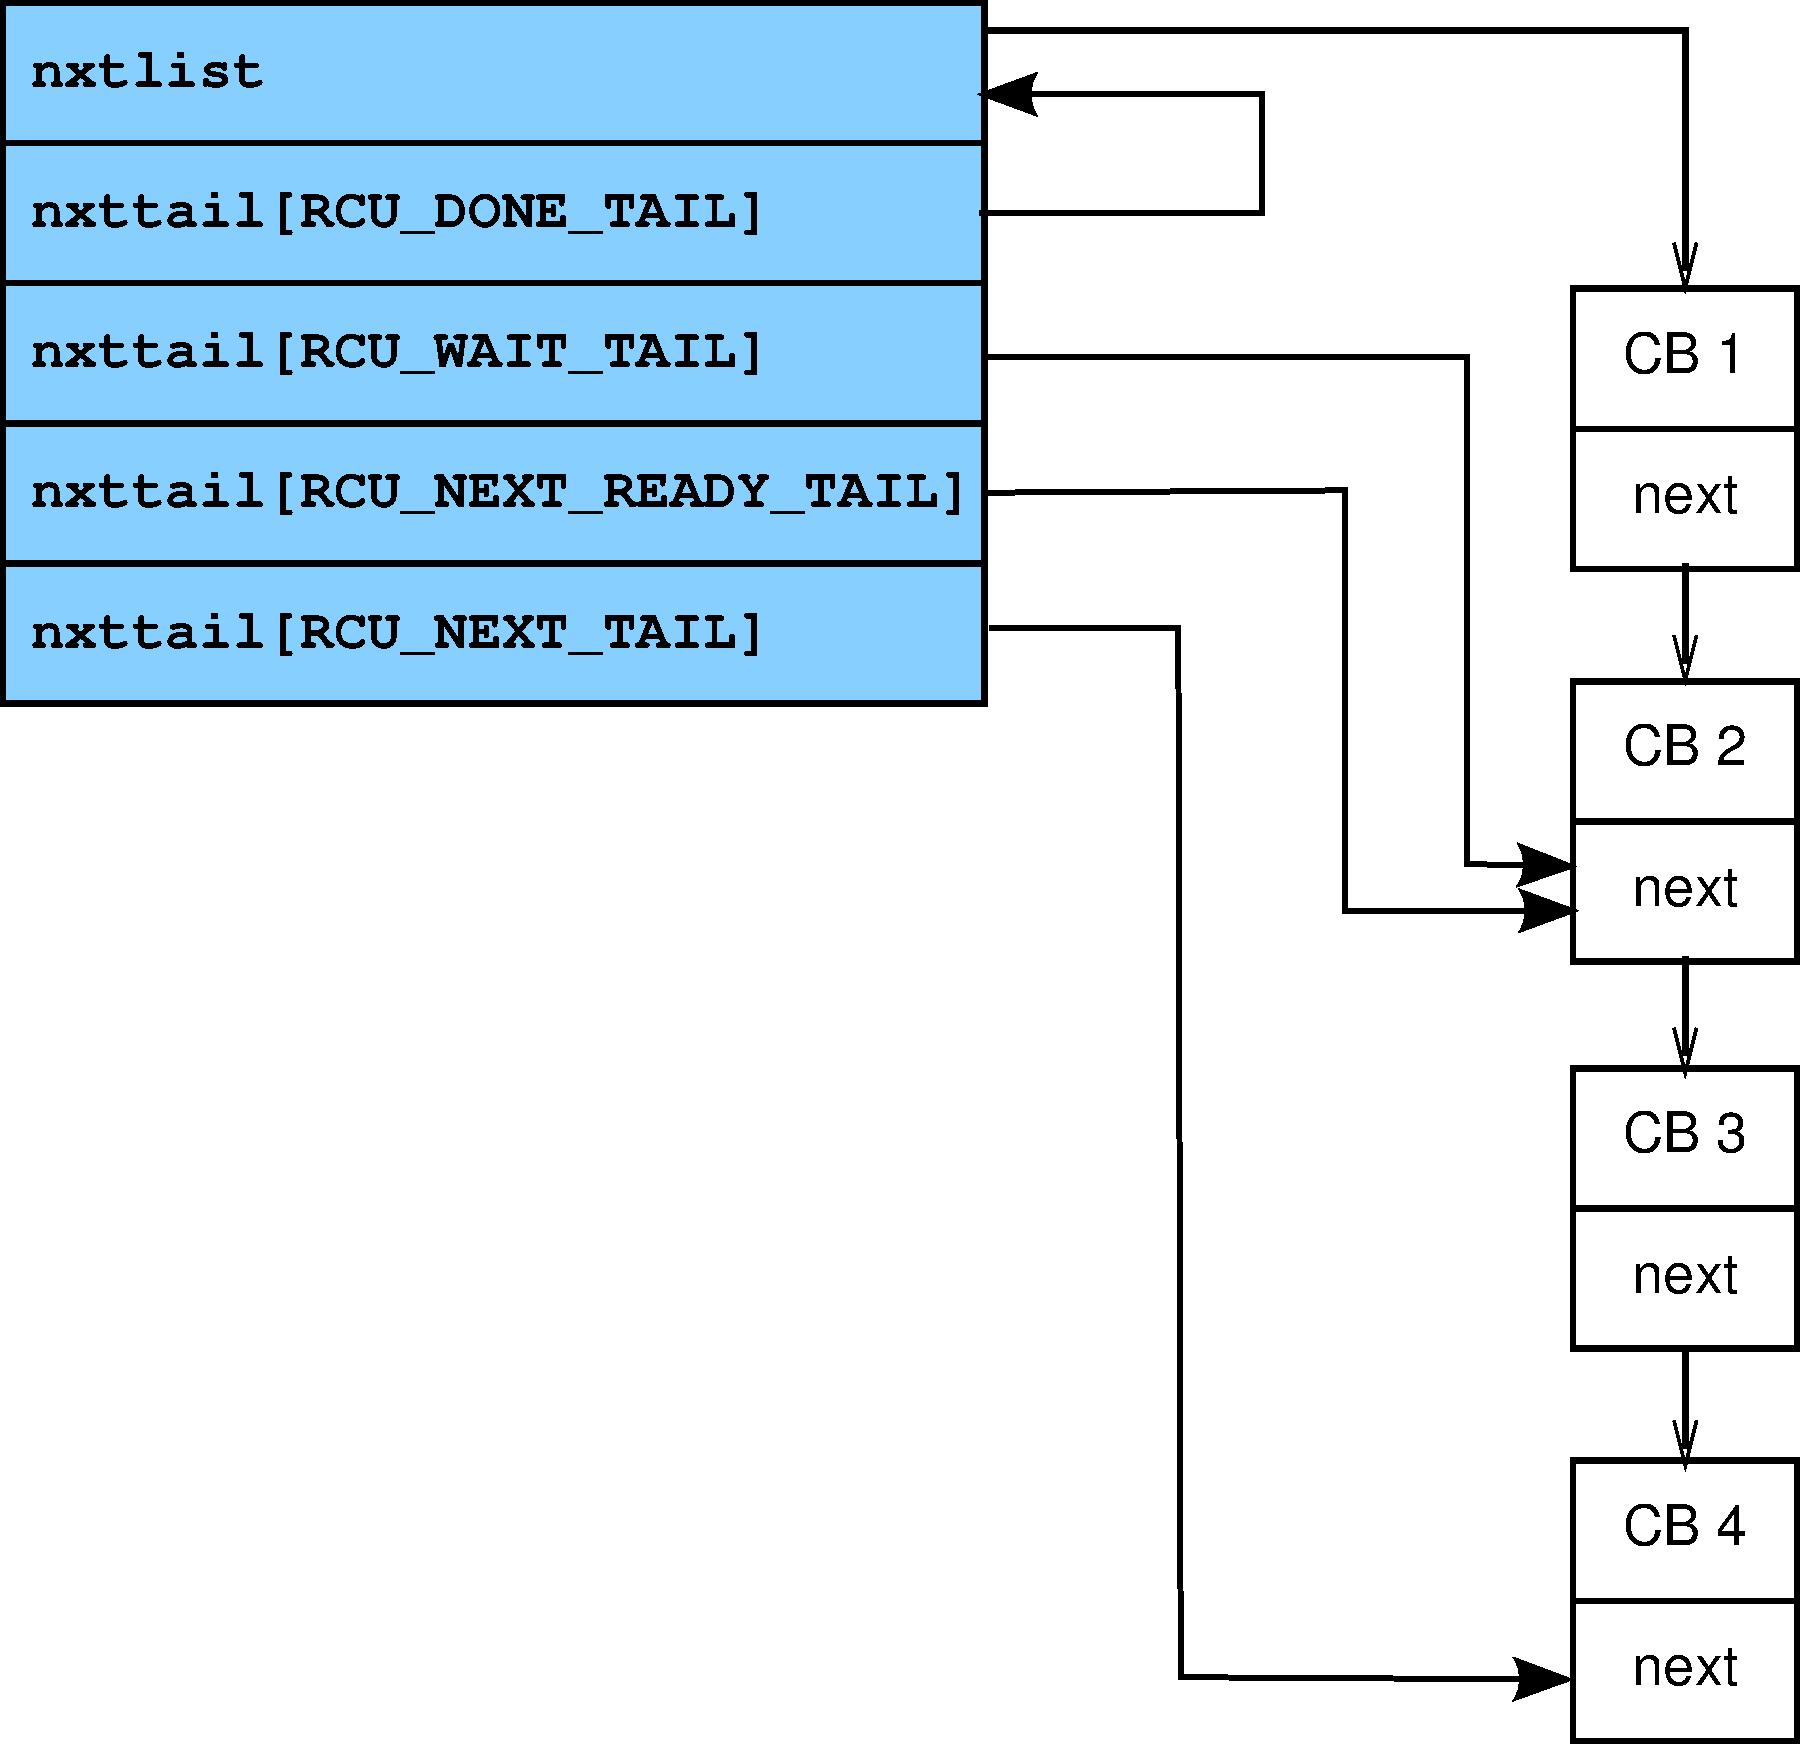
\includegraphics[scale=0.25]{rcu_data_callbacks.pdf}
\caption{Callback Queuing in \co{rcu_data}}
\label{fig:rcu_data_callbacks}
\end{figure}

%\comment{Lihao: since we don't model callbacks, only describe them briefly and add a reference
%to save space for the experiments section which is the main contribution of this paper. 
%Do the same for discussion of preemptible RCU.}
\subsubsection{RCU Callbacks}
The \co{rcu_data} structure manages RCU callbacks using a \co{->nxtlist}
pointer tracking the head of the list and an array of \co{->nxttail[]}
tail pointers that form a four-segment list of
callbacks~\cite{LaiJiangshan2008NewClassicAlgorithm}, with
each element of the \co{->nxttail[]} array referencing the tail of the
corresponding segment, as shown in Figure~\ref{fig:rcu_data_callbacks}.
The segment ending with \co{->nxttail[RCU_DONE_TAIL]} (the ``\co{RCU_DONE_TAIL}
segment'') contains callbacks
handled by a prior grace period that are therefore ready to be invoked.
The \co{RCU_WAIT_TAIL} and \co{RCU_NEXT_READY_TAIL} segments 
contain callbacks waiting for the
current and the next grace period, respectively.
Finally, the \co{RCU_NEXT_TAIL} segment contains
callbacks that are not yet associated with any grace period.
%
The \co{->qlen} field counts the total number of callbacks, and
the \co{->blimit} field specifies the maximum number of RCU callbacks
that may be invoked at a given time, thus limiting response-time
degradation due to long lists of callbacks.\footnote{
	Workloads requiring aggressive real-time guarantees should use
	callback offloading, which is outside of the scope of this paper.}

Back in Figure~\ref{fig:rcu_data_callbacks}, the
\co{->nxttail[RCU_DONE_TAIL]} array element references \co{->nxtlist}, 
which means none of the callbacks are ready to invoke.
The \co{->nxttail[RCU_WAIT_TAIL]} element references callback 2's \co{->next}
pointer, meaning that callbacks CB~1 and CB~2 are waiting for the current
grace period.
The \co{->nxttail[RCU_NEXT_READY_TAIL]} element references that same \co{->next}
pointer, meaning that no callbacks are waiting for the next grace period. 
Finally, the callbacks between the \co{->nxttail[RCU_NEXT_READY_TAIL]} and
\co{->nxttail[RCU_NEXT_TAIL]} elements (CB~3 and CB~4)
are not yet assigned to a specific grace period.
The \co{->nxttail[RCU_NEXT_TAIL]} element always references either
the last callback or, when the entire list is empty, \co{->nxtlist}.

Cache locality is promoted by invoking callbacks on the CPU that registered
them.
For example, RCU's update-side primitive 
\co{synchronize_rcu()} appends callback \co{wakeme_after_rcu()} to the end
of the \co{->nxttail[RCU_NEXT_TAIL]} list in the current CPU 
(Section \ref{sec:update_api_impl}). 
They are advanced one segment towards the head of the list (via \co{rcu_advance_cbs()}) 
when the CPU detects the current grace period has ended, which is indicated 
by the \co{->completed} field of the CPU's \co{rcu_data} structure being one
smaller than its counterpart in the corresponding leaf \co{rcu_node} structure.
The CPU also periodically merges the \co{RCU_NEXT_TAIL} segment into the
\co{RCU_NEXT_READY_TAIL} segment by calling \co{rcu_accelerate_cbs()}.
In a few special cases, the CPU merges the \co{RCU_NEXT_TAIL} segment
into the \co{RCU_WAIT_TAIL} segment, bypassing the \co{RCU_NEXT_TAIL}
segment.
This optimization applies when the CPU is starting a new grace period.
It does \emph{not} apply when a CPU notices a new grace period
because that grace period might well have started before
the callbacks were added to the \co{RCU_NEXT_TAIL} segment.
%\comment{Lihao: why can't we invoke *all* callbacks when starting a new 
%grace period? Isn't it true that all pre-existing read-side critical
%sections, i.e.~those start before callbacks are registered in \co{->nxttail} 
%(in particular \co{wakeme_after_rcu} in \co{->nxttail[RCU_NEXT_TAIL]}), 
%have finished?}
%\comment{Paul: In theory, we could, but in practice doing this would
%have several disadvantages:
%(1) All callbacks would be invoked by the grace-period kthread, and
%large systems could generate more callbacks than a single CPU could
%keep up with, which would delay subsequent grace periods and possibly
%even run the system out of memory.
%(2) Running all the callbacks at once could degrade real-time response.
%(3) Running callbacks on a different CPU than the one that registered
%them would decrease locality, increasing cache-miss rates, thus degrading
%performance.
%(4) This would require that atomic instructions be used when registering
%callbacks (as they are for no-CBs CPUs), further degrading performance.
%In addition, we could only invoke callbacks in the \co{RCU_NEXT_TAIL}
%segment, because callbacks in the later segments
%(\co{RCU_NEXT_READY_TAIL}, \co{RCU_WAIT_TAIL}, and
%\co{RCU_DONE_TAIL} might well have been queued \emph{after} the
%recently-completed grace period started.}
%
This is a deliberate design choice: It is more important for the CPUs
to operate independently (thus avoiding contention and synchronization
overhead) than it is to decrease grace-period latencies.
In those rare occasions where low grace-period latency is important,
the \co{synchronize_rcu_expedited()} should be used.
This function has the same semantics as does \co{synchronize_rcu()},
but trades off efficiency optimizations in favor of reduced latency.
% Lihao: this is where the callback of RCU's update API register? 
% Paul: Yes, call_rcu() appends the callback to the end of the current
% CPU's RCU_NEXT_TAIL list.  Ignoring callback offloading for the moment.
% Lihao: we don't model QS forcing and offline CPUs
% Paul: Nor are you modeling callback offloading.  Which is fine, just calling
% it out.  ;-)

Each RCU callbacks is an \co{rcu_head} structure which has a
\co{->next} field that points to the next callback on the list and
a \co{->func} field that references the function to be invoked at the
end of an upcoming grace period.



